\documentclass[]{aiaa-tc}

\usepackage{authblk}
\usepackage{booktabs}
\usepackage{hyperref}
\usepackage{subfig}
\usepackage{amsmath}
\usepackage{amssymb}
\usepackage{pdflscape}
\usepackage{appendix}
\usepackage{pdfpages}


\newcommand{\bigcell}[2]{\begin{tabular}{@{}#1@{}}#2\end{tabular}}

%\usepackage[margin=3cm]{geometry}

\setlength\extrarowheight{5pt}

\bibliographystyle{aiaa}


\newcommand{\f}{\frac}
\newcommand{\p}{\partial}
\newcommand{\ds}{\displaystyle}
\newcommand{\mb}{\mathbf}
\newcommand{\mbs}{\boldsymbol}


\begin{document}

  %\maketitle

  \vspace{4em}
  \begin{center}
    A proposal to the NASA ARMD Team Seedling Program: 
    \vspace{2em}

    {\Huge Coupled Aero­-Structural-Propulsive­ Design of an Ultra­Light, Highly Flexible, Human Powered Aircraft}

    \vspace{2em}
    submitted to the NASA Aeronautics Research Institute by: 

    \vspace{3em}
    \begin{figure}
        \centering
        
\includegraphics[width=.5\textwidth]{images/seedling_logos}
    \end{figure}
    \vspace{3em}


  \end{center}


  \begin{tabular}{l l}
    Principal Investigator & Justin S. Gray; NASA Glenn Research Center, Propulsion Systems Analysis Branch \\ 
    & \\
    Co-Investigators & Dr. Juan Alonso; Stanford University, Department of Aeronautics and Astronautics \\
                     & Dr. Graeme Kennedy; Georgia Institute of Technology, School of Aerospace Engineering \\ 
                     & Dr. Todd Reichert; Vice President of Aerodynamics, AeroVelo Inc. \\
    & \\ 
    Team Members & Cameron Robertson; Vice President of Structures, AeroVelo Inc. \\ 
                 & Jeffrey Chin; NASA Glenn Research Center, Propulsion Systems Analysis Branch \\
                 & Kevin Reynolds; NASA Ames Research Center, Intelligent Systems Branch \\
  \end{tabular}

  \newpage

  \section{Introduction}

    The Fundamental Aeronautics Program has identified \textbf{Ultra Efficient Commercial Vehicles} as 
    a key research thrust. A number of concepts have been proposed along those lines, such as 
    the MIT D8 double­-bubble and the Boeing SUGAR­-High truss­-braced wing. These aircraft rely on 
    very high­-aspect ratio, extremely flexible wings to help achieve very low energy consumption. 
    Long endurance solar sensorcraft, being proposed by companies such as General Atomics and 
    Scaled Composites, share a similar approach to minimizing energy consumption by leveraging highly 
    flexible wings. This begs the question, \textbf{``How does aircraft design change to take full 
    advantage of highly flexible structures?''} The Vision 2030 CFD study also highlights the 
    design of highly flexible wings as a modeling grand challenge problem. That study specifically 
    highlights the need for highly multidisciplinary, tightly coupled design process with high 
    fidelity tools to address this grand challenge.

    Aircraft empty weight reduction is a major driving factor pushing designs toward highly flexible structures. 
    While lower structural weight helps to achieve lower energy consumption it also tends to result in very large 
    deflections and highly non-linear structural responses. These characteristics mean that 
    structural considerations play a major role in the overall aircraft design, and have been shown to be a primary 
    concern for aircraft stability\cite{heliosfailure_2007}. Thus it is interesting to consider the question, 
    \textbf{``Could structural health monitoring technologies be used to enable lighter 
    weight structures?''}, to address the \textbf{Real­-Time System­-Wide Safety Assurance} thrust. 

    One of the major challenges associated with designing highly flexible wings is that the as-flown configuration 
    is dramatically different than the as-built configuration (jig shape). With modern aeroelastic techniques, 
    we can now design more conventional wings taking this into account~\cite{Kennedy:2014:tacs-tripan, Kennedy:2012:CMC, 
      Kennedy:2014:High-aspect-ratio}. However, highly flexible
    structures bring new challenges that need to be addressed. Besides the non-linear structural 
    response these wings also tend to have different load distributions from conventional wings. Many of the concepts 
    are electric aircraft with propellers spread out across the wing for distributed propulsion. This can have not only a 
    structural impact, but also an aerodynamic and controllability impact as well. These aspects push the 
    limits of todays most advanced high-fidelity aeroelastic design techniques, which currently rely on linear structural 
    models, don't account for any propulsion interactions, and don't easily handle constraints on dynamic behavior. 

    Although tools currently exist to address each one of the various modeling challenges, there is not yet a well 
    established method to integrating them all into a cohesive system model and then applying that model to an actual 
    aircraft design process. This proposal outlines a unique opportunity for NASA to fill this capability gap
    via an aircraft design and flight testing effort done in close collaboration with AeroVelo Inc., Georgia 
    Institute of Technology, and Stanford University. In 2013 AeroVelo won the Sikorski Human Powered Helicopter Prize. 
    Their next human powered aircraft will be built to conquer the Kremer Marathon Challenge; fly a 
    human powered aircraft 26.1 miles in under 1 hour. They have invited a NASA led team of researchers to 
    participate in this project. 

    A human powered aircraft designed for the Kremer Marathon Challenge makes an excellent test case for the 
    wide range of modeling and design challenges associated with highly flexible wings. 
    The only available power is that of the humans on board, and each one can provide about the 
    same amount of power as a cordless drill. In order to reach the speeds necessary, multiple people will be required. 
    Figure \ref{fig:aerovelo-concept} is the initial AeroVelo concept, which includes three pilots spread across the wing
    span with three propellers. Spreading the pilots out over the wing span yields a distributed load profile, 
    which must be supported by a very light weight and extremely flexible structure. Weight is not the only 
    key design consideration either. To keep aerodynamic drag low, it is critical to maintain laminar flow 
    over as much of the wing as possible. 

    \begin{figure}
        \centering
        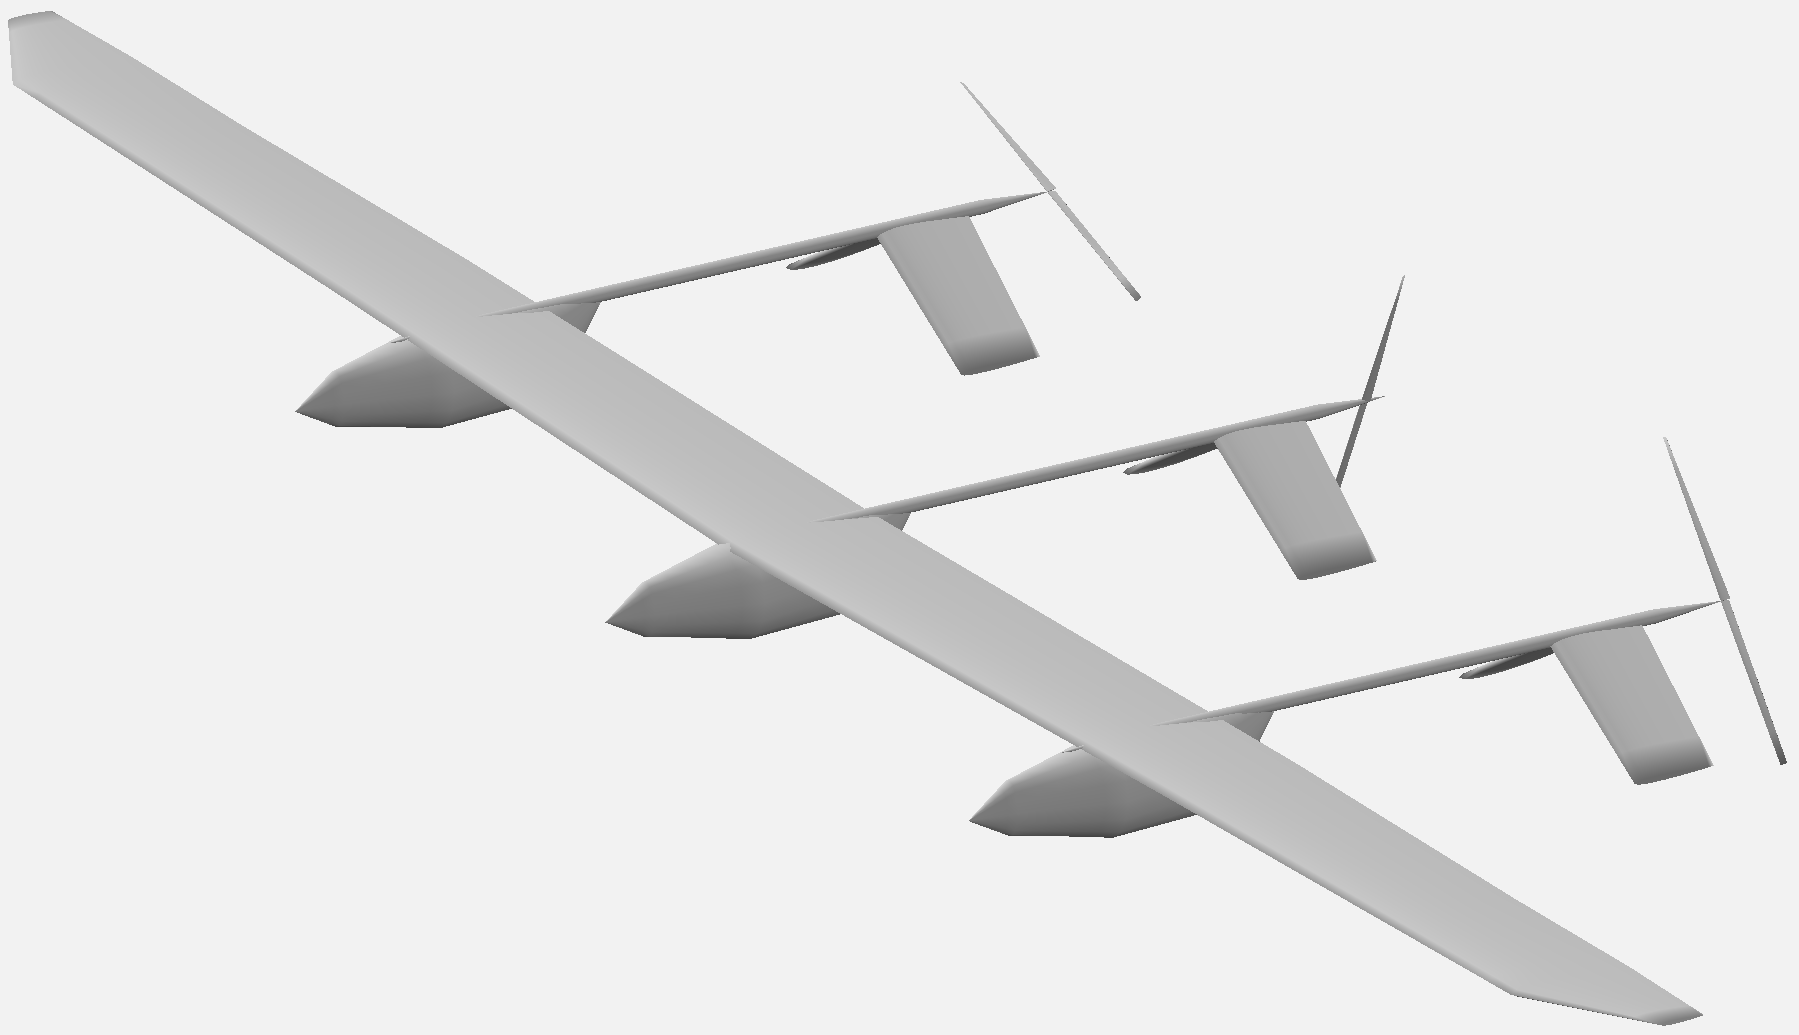
\includegraphics[width=.5\textwidth]{images/vsp_concept_solid}
        \caption{AeroVelo concept of 3 pilot human powered aircraft for the Kermer Marathon Aircraft}
        \label{fig:aerovelo-concept}
    \end{figure}

    The combination of low speed flight, very low available power, distributed propulsion, and highly 
    flexible span-loaded structures makes this human powered aircraft an excellent analog for 
    high altitude, long endurance aircraft. Hence all of the tools and methods developed under 
    this effort will be directly applicable to that class of aircraft. But by working with a human powered 
    aircraft, we are able to achieve a lower cost, rapid feedback environment to develop and validate these 
    new methods. Then later efforts can quickly applye the new methods to other types of aircraft like the D8
    or HALE concepts. 

    In phase one of this effort, the analysis tools and coupled design environment will be built and 
    the detailed design of the marathon aircraft will be completed. In addition, sub-scale testing will be 
    performed to validate structural models and construction techniques. In phase two of the effort
    the aircraft will be built, tested, and flown to attempt the Kremer Marathon Challenge. The aircraft will be 
    used as a flying test bed to collect further structural and aerodynamic validation data. All the data collected, 
    all of the models, and the final detailed design will be released publicly under an open-source license.

  \section{Objectives and Technical Approach}

    The overall objective of this work is to design, test, and fly a human powered aircraft, 
    capable of flying 26.1 miles in under 1 hour using state-of-the-art multidisciplinary 
    design optimization techniques. The design will be performed with fully coupled
    aerodynamic, non-linear structural, and propeller models. Working in the context of 
    a full aircraft design process, from conceptual all the way to detailed design, 
    provides a unique opportunity to apply multidisciplinary optimization methods and validate
    the results within a vary small time frame. 

    Phase one of the work will focus on the design of the aircraft. NASA Glenn Research Center, 
    NASA Ames Research Center, Stanford, and the Georgia Institute of Technology will be responsible 
    for collaboratively developing the propulsion, aerodynamic, and structural analysis 
    models needed as well as integrating them together for perform the coupled analysis. AeroVelo will
    use the models to perform the conceptual, preliminary, and detailed design of the actual marathon 
    aircraft in very close collaboration with the other partners. NASA Glenn Research Center, 
    The Georgia Institute of Technology, and AeroVelo will all collaborate on a set of structural validation 
    tests designed to validate the tool sets and construction methods needed for the aircraft. 

    \subsection{Model Integration (Glenn)}

    NASA Glenn will be responsible for managing the integration of the various analyses into 
    a single system model via the OpenMDAO framework. OpenMDAO provides advanced 
    capabilities for high-fidelity code coupling. These capabilities will be leveraged to combine the geometry,
    propeller, wing aerodynamics, and structural models into a single coupled aircraft model. The aircraft 
    model will the be used as a design tool by AeroVelo to facilitate the actual design process. 
    Figure ~\ref{fig:n2} shows details of how the multidisciplinary coupling will be set up. The aerodynamics 
    and structures disciplines will both be implemented using high fidelity models. The propeller modeling 
    will be accomplished with a combination of low and high fidelity models. The use of high fidelity models 
    will pose a significant challenge to the design process. Airfoils must be designed independently along the propeller and
    across the entire wing . In addition, material thickness throughout the structure
    will be sized independently. The combination of aerodynamic and structural design variables 
    can easily number in the 100's to 1000's. With such a large design space, gradient based optimization 
    combined with adjoint analytic derivatives are the most effective tool for navigating the design space. 

    \begin{figure} \centering
        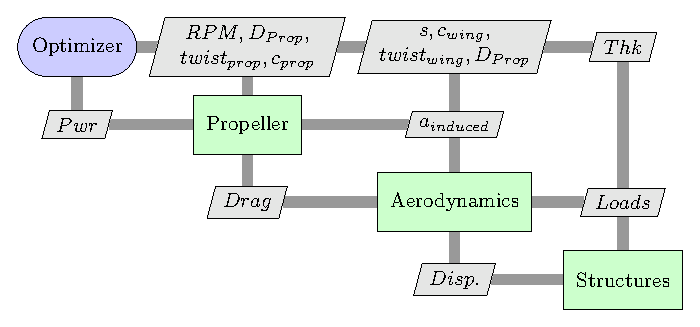
\includegraphics[width=.75\textwidth]{xdsm/overall}
        \caption{Data flow for the aircraft design process, with coupling between the propeller and aerodynamics models 
        and between the aerodynamics and structural models. }
        \label{fig:n2}
    \end{figure}

    Because of the size of the design space, and larger number of coupled disciplines, OpenMDAO's built in support for 
    automatic system level coupled derivatives will be key to building the aircraft level model. OpenMDAO allows for 
    pure analytic or semi-analytic derivatives, using both forward and adjoint formulation. The effectiveness of OpenMDAO's 
    derivatives capability has been successfully demonstrated on to two different design problems that are similar in complexity 
    and scale to the proposed human powered aircraft design: A small satellite design and an aero-structural 
    wind turbine design\cite{gray2014derivatives}. The small satellite design problem had over 25,000 design variables 
    and over 30 disciplines. This problem demonstrated OpenMDAO's capabilities to solve problems of very large scale with adjoint 
    derivatives. The aero-structural design of a wind turbine was a very different problem. It used a mixture of analytic and 
    finite difference gradients with a complex system level model considering aerodynamics, structures, and economics. 
    This problem showed that even when applying finite difference to some of the disciplines for gradients, the analytic 
    derivative approach yielded a factor of 5 reduction in compute costs. This previous work demonstrates the 
    value of OpenMDAO's analytic derivatives capability and highlights why it will be a central feature in the design 
    optimization for a human powered aircraft. 

    By using the OpenMDAO framework, the modeling methods will be built in modular fashion that will allow a wide range of
    different analysis tools to be used. This will help extend the applications of the work to other types of aircraft beyond the 
    initial human powered aircraft. 

    \subsection{Aerodynamic Modeling (Stanford / Ames)}

    Stanford's SU2 CFD tool, will be used for the aerodynamic analyses of both the wing and 
    the propellers. SU2 has been successfully applied to the design of propeller systems 
    and has support for actuator disk boundary conditions that will be needed to implement 
    the coupled wing­-propeller design process. It has been demonstrated to work in the low 
    Mach conditions that will be seen by this aircraft. It also provides adjoint derivatives 
    which are fundamental to the application of state­-of-­the-­art gradient based design 
    optimization methods. Researchers at Stanford will be responsible for building for developing 
    the aerodynamic models of the wing and will collaborate with NASA Ames on developing the 
    propeller models. In addition they will provide support for integrating SU2 into the OpenMDAO 
    framework. 

    \subsubsection{Propeller Analysis (Ames)}
        \begin{itemize}
            \item SU2 can be applied using the rotating reference frame features for efficient high fidelity propeller design
            \item Lower fidelity tools may be even more efficient and could be highly accurate with good 2d airfoil data. Andrew Ning's 
            CCBlade is a good option. 
        \end{itemize}

    \subsubsection{Wing \& Fueselage Analysis (Stanford)}
        \begin{itemize}
            \item Laminar flow is a key design requirement for both the wing and the pilot fairings. An inverse design approach can be employed 
            by specifying a desired pressure distribution. 
            \item TriPan is a lower fidelity option that also provides gradients and could possibly be employed to reduce computational cost. It might make sense to set things up so that SU2 and Tripan could be used interchangeably. 
        \end{itemize}

    \subsubsection{Wing-Propeller Coupling (Glenn/Stanford)}
        \begin{itemize}
            \item SU2 actuator disks for coupling
        \end{itemize}

        \subsection{Structural Modeling (GaTech)}

The modeling and design of slender lightweight flexible structures for
human and electric-powered aircraft requires specialized tools due to
the strongly-coupled multidisciplinary physics that govern these
vehicles. These requirements will be met, in part, by performing the
structural modeling with the Toolkit for Analysis and of Composite
Structures (TACS). TACS has the necessary capabilities to develop a
tightly integrated multidisciplinary framework for dynamic and static
aeroelastic design optimization. These advanced capabilities include
adjoint derivative evaluation and efficient parallel load and
displacement transfer required for coupled aeroelastic analysis and
design.  In addition, TACS also has support for iso-geometric elements
which will reduce the overall computational cost of the structural
analysis. Researchers at the Georgia Institute of Technology will be
responsible for building the structural models and providing support
for integrating them into the OpenMDAO framework.

Isogeometric analysis (IGA) techniques are attractive since they
enable CAD-compatible geometry modification while retaining the
advantages of high-order structural analysis. IGA methods utilize the
underlying b-spline basis functions from the geometry model for
displacement interpolation, producing smooth and accurate displacement
and stress solutions. The improved smoothness properties of the stress
distribution from IGA shells smooths the design space for
stress-constrained mass minimization with gradient-based design
optimization.

Integration of aerodynamic, structural, and dynamic aeroelastic design
criteria will be required to achieve a lightweight design that
satisfies all design constraints. We will integrate the IGA analysis
within our structural analysis and design code called the Toolkit for
the Analysis of Composite Structures
(TACS)~\cite{Kennedy:2014:TACS}. TACS is a parallel finite-element
code for large-scale structural analysis and design optimization with
sophisticated gradient evaluation capabilities. TACS is also designed
for multidisciplinary analysis and design optimization of composite
structures, with an existing load and displacement transfer scheme
designed for efficient parallel computations.

\subsubsection{Nonlinear structural modeling}

In this work, we will utilize a third-order isogeometric shell element
for nonlinear structural analysis and design.  This element balances
the computational costs of analysis and gradient evaluation, with the
superior accuracy of higher-order elements. However, quadratic
b-spline elements are susceptible to both shear and membrane
locking~\cite{Babuska:1992:OLR, Chapelle.Bathe}. Therefore, to
alleviate this locking issue, we utilize a mixed-interpolation of
tensorial (MITC) approach~\cite{Dvorkin:1984:CMB, Bucalem:1993:HOM}.

\begin{figure}[h]
  \centering
  \subfloat[Shell formulation]{
    \label{fig:shell-geometry}
    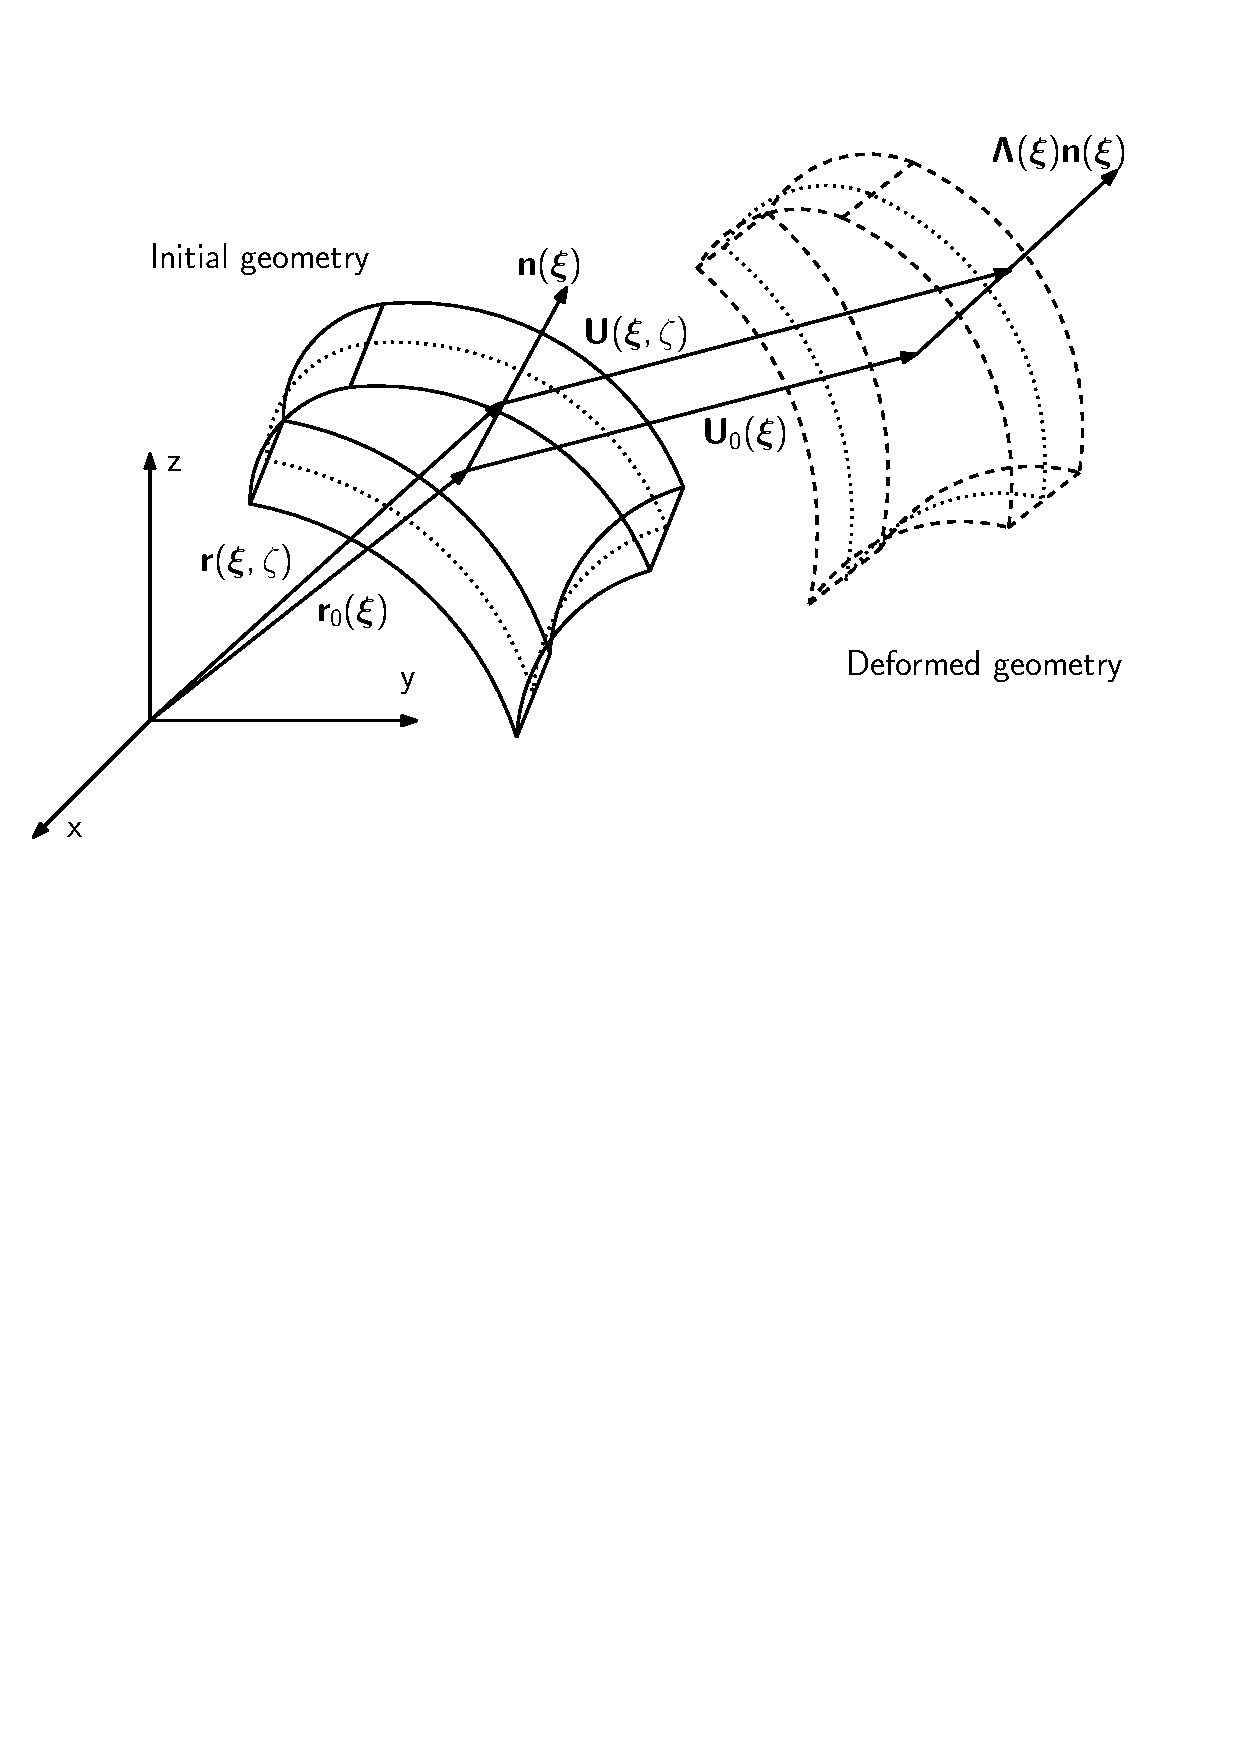
\includegraphics[width=0.4\textwidth]{images/shell_formulation}}
  \subfloat[MITC scheme]{
    \label{fig:mitc-formulation}
    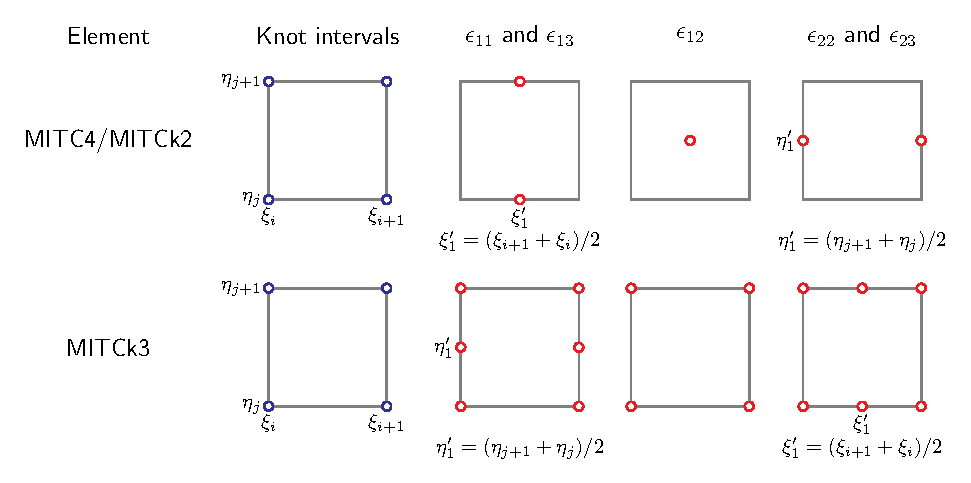
\includegraphics[width=0.6\textwidth]{images/mitc_iga}}
  \caption{The large rotation shell formulation and the b-spline
    compatible MITC scheme.}
  \label{fig:shell-figs}
\end{figure}

The formulation of a general shell element for geometrically nonlinear
analysis is extremely challenging. The elements in TACS use a
degenerated solid approach in which each shell element is formulated
by reducing the full three-dimensional equations of elasticity to the
mid-surface using shell-theory-like assumptions about the distribution
of the displacements through the thickness~\cite{Ahmad:1970:ATS,
  Bathe:1980:GMN, Parisch:1978:GNA, Hughes:1981:NFE}.  The degenerated
solid analysis is mathematically equivalent to a shell theory
formulation under similar same modeling
assumptions~\cite{Buechter:1992:STD}.  We use an explicit integration
of the strain energy through the thickness, enabling the direct use of
the classical first-order deformation theory (FSDT) constitutive
relationships~\cite{Milford:1986:DIF, Buechter:1992:STD}. The
in-plane drilling degree of freedom is included and a penalization
technique is used to ensure compatibility with the in-plane
displacements~\cite{Hughes:1989:DDF, Simo:1992:FFE,
  Fox:1992:DRF}. This formulation facilitates shell-shell
intersections.

The initial, undeformed shell geometry is represented in terms of the
mid-surface vector, $\mb{r}_{0}(\mbs{\xi}) \in \mathbb{R}^{3}$, and
the unit normal, $\mb{n}(\mbs{\xi})$, that are written in terms of the
local shell coordinates $\mbs{\xi}$. The through-thickness coordinate
is given by $\zeta$. The entire shell volume can be expressed as
follows:
%
\begin{equation} 
  \mb{r}(\mbs{\xi}, \zeta) = 
  \mb{r}_{0} + \zeta \mb{n}, 
  \qquad \mbs{\xi} \in \Omega \subset \mathbb{R}^{2}, \qquad.
  \label{eqn:mid-surface}
\end{equation}
Figure~\ref{fig:shell-geometry} illustrates the initial and the deformed
configurations of a shell segment. 

For the shell model, we use kinematic assumptions that are consistent
with a large-displacement, finite-rotation shell. In particular, we
use a director-field representation~\cite{Simo:1989:SRG1}, such that
the normal deforms as, $\mb{d} = \mbs{\Lambda} \mb{n}$, where
$\mbs{\Lambda} \in SO(3)$ is a rotation matrix. The through-thickness
displacement is written in terms follows:
%
\begin{equation*}
  \label{eqn:displacement-field}
  \mb{U}(\mbs{\xi}, \zeta) = \mb{U}_{0} + \zeta (\mbs{\Lambda} - \mb{I}) \mb{n}.
\end{equation*}
where $\mb{U}_{0}$ are the mid-surface displacements and $\mbs{\Lambda}$ is
a rotation matrix.

For the finite-element implementation, we utilize an isogeometric
analysis (IGA) approach. IGA methods have the advantages of
higher-order displacement and stress prediction accuracy. In the IGA
method, the basis functions are b-spline functions which are defined
using the Cox-de~Boor recursion formula as follows~\cite{NURBSbook}:
%
\begin{equation}
  \label{eqn:b-spline-basis}
  \begin{aligned}
    N_{i,p}(u) & = \f{u - u_{i}}{u_{i+p} - u_{i}} N_{i,p-1}(u) + \f{u_{i+p+1} - u}{u_{i+p+1} - u_{i+1}}N_{i+1,p-1}(u) \\
    N_{i,0}(u) & = \left\{ 
      \begin{array}{l} 
        1 \qquad \text{if}\;\; u_{i} \le u < u_{i+1} \\
        0 \qquad \text{otherwise}
      \end{array} \right.
  \end{aligned}
\end{equation}
%
These basis functions are used to both interpolate the
mid-surface~\eqref{eqn:mid-surface} and construct the displacement and
rotation fields~\eqref{eqn:displacement-field}. Since we use
third-order, bi-quadratic b-spline meshes, our formulation is
susceptible to shear and membrane-locking. To alleviate these issues,
we therefore utilize an mixed interpolation of tensorial components
(MITC) approach that utilizes the tying-point scheme shown in
Figure~\ref{fig:mitc-formulation}.  Note that the scheme for
second-order, bi-linear b-spline surfaces degenerates to the classical
MITC4 shell element.

\subsubsection{Aeroelastic load and displacement transfer}

For this project, our team will develop a coupled aeroelastic design
capability between TACS and $\text{SU}^2$, using existing parallel
load and displacement transfer
techniques~\cite{Kennedy:2014:tacs-tripan}. 

\begin{figure}
  \centering
  \subfloat[Displacement transfer rigid links]{
    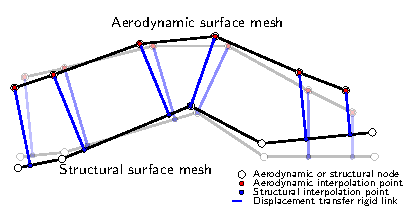
\includegraphics[width=0.5\textwidth]{images/rlink_displaced}
  \label{fig:rigid-link-displacement}}
  \subfloat[Load transfer rigid links]{
    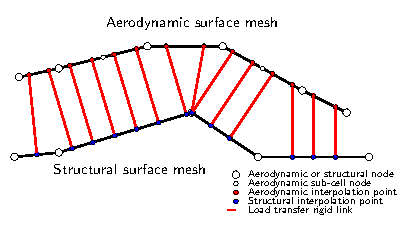
\includegraphics[width=0.5\textwidth]{images/rlink_displacement}
    \label{fig:rigid-link-force}}
  \caption{Load and displacement transfer rigid links for a
    second-order finite-element mesh.}
\end{figure}

This load and displacement transfer technique is a consistent method
based on the method of virtual work. The method works by extrapolating
the displacements from the structural surface to the aerodynamic
surface using both a series of rigid links. These rigid links are
constructed by finding the closest structural surface point to each
aerodynamic mesh location. The rigid links for displacement
extrapolation are illustrated in
Figure~\ref{fig:rigid-link-displacement}.

Next, the aerodynamic surface loads are transferred through a
consistent and conservative technique based on the rigid-link
extrapolation. This integration is computed as follows:
\begin{equation}
  \begin{aligned}
    \delta\, W & = q \int_{S_{A}} \, C_{p} \, \hat{\mb{n}}^{T} \delta\mb{u}_{A} \, \mathrm{d}S \\
    & = q\int_{S_{A}} \, C_{p} \left( \hat{\mb{n}}^{T} \delta \mathbf{u}_{S} -
    \left( \hat{\mb{n}}\times \mb{r}_{SA} \right)^{T} \delta \mbs{\theta}_{S} \right) \, \mathrm{d}S,
  \end{aligned}
  \label{eqn:method-virtual-work}
\end{equation}
where $q$ is the dynamic pressure, $C_{p}$ is the surface pressure
coefficient $\mb{u}_{A}$ and $\mb{u}_{S}$ are the displacements at the
aerodynamic and structural surfaces, $\mbs{\theta}_{S}$ is the
rotation at the structural surface, $\mb{r}_{SA}$ is the rigid-link,
and $\hat{\mb{n}}$ is the normal defined on the deformed aerodynamic
surface.

We approximate the integral~\eqref{eqn:method-virtual-work} by adding the
contributions from each aerodynamic surface cell using a two-part
numerical quadrature rule. First, we split quadrilateral cells based
on a specified characteristic length scale into a series of
subquadrilaterals. The characteristic length scale is selected to
match the length scale of the average finite-element within the
structural model. If any side of the quadrilateral exceeds the
characteristic length scale, we split the cell along that edge into
multiple subcells. Next, on each subcell we use a Gauss quadrature
scheme that matches the order of accuracy required by the underlying
finite-elements. For each quadrature point within each subcell, we
compute a rigid link from the quadrature point to the structural
surface in an analogous manner to the displacement transfer
scheme. This two-level quadrature rule is effective at smoothly
transferring loads to the finite-element mesh even in the presence of
high-aspect-ratio surface cells. Figure~\ref{fig:rigid-link-force}
illustrates the load transfer scheme including the subcell refinement
step.

\subsubsection{Illustration of the IGA modeling capabilities}

    % \subsection{Structural Dynamics Modeling (Glenn/AeroVelo)}

    % Structual dynamics are a very important design consideration for aircraft with highly flexible wings. Large spans and low mass
    % combine to make dynamic bending modes and structural response to control inputs both key constraining factors. NASA's Helios 
    % aircraft experienced a catastrophic failure related to unexpected structural dynamic response, clearly demonstrating the importance
    % of accouting for this phenomenon in these types of aircraft. 
    % However, directly modeling it with high fidelity codes is currently computationally infeasible in an optimization context. Never the less, 
    % some analysis needs to be included in the system model to account for these issues. Mark Drela's ASwing code is a lower fidelity 
    % coupled aero-structural analysis tool that can account for the non linear structural dynamics using a beam based method\cite{DrelaASWING}. This tool was specifically built for this type of application to be used in a rapid iteration design process. It  
    % will be coupled in to the overall system model. 

    % Although ASwing does not provide analytic derivatives, its low computational cost makes it feasible to use finite difference to 
    % get the disciplinary derivatives. These can then be combined with the other disciplines by OpenMDAO's mixed derivatives capabilities
    % to maintain the high efficiency of the overall design optimization. 

    \subsection{Aircraft Design (AeroVelo)}

    AeroVelo will be responsible or the actual design and construction of the aircraft using the tools developed 
    by the other team members. They will also be responsible for building the structural test articles and designing 
    the structural validation tests. After the attempt has been made, NASA will be given access to 
    the aircraft to perform additional test flights to collect data. 

    % \subsection{Wind Tunnel Testing}
    %     \begin{itemize}
    %         \item Expect airfoils to have a chord of about 2 feet. Flight speeds will be about 26 mph (40 feet/sec). Can we find a wind tunnel 
    %         that can test an article of that size at such slow speeds? 
    %         \item Another option would be to build a small test wing and fly it on a drone. Ames has the ability to rapidly prototype this kind 
    %         of drone and could provide actual flight tests. I suspect this would be a lower cost solution, but could 
    %         present measurement challenges. 
    %     \end{itemize}

    \subsection{Structural Testing \& Model Validation}
        \begin{itemize}
            \item CFOSS system for structural tests?? 
            \item What kind of measurements are necessary to validate the codes? 
            \item What kind of measurements are necessary to validate the design? 
        \end{itemize}



  \section{Innovation \& Impact}

    The Kremer marathon challenge was established in 1959, and has remained unmet for the last 55 years. 
    Successful completion of work proposed here could result in could result in finally achieving this very challenging
    aviation milestone. AeroVelo is already well know for their 2013 claiming of the Sikorski Prize with their Atlas 
    Human Powered Helicopter. Their stated mission is ``to inspire the public and youth, tackle the impossible, and 
    challenge conventional design by doing more with less.'' Partnering with AeroVelo for this work will bring a significant
    amount of visibility to the results of this work and help raise awareness of the public benefit from NASA's advanced 
    multidisciplinary design research. 

    Additionally, the work will significantly advance state-of-the art for design methods of highly flexible wings. 
    A fully coupled high-fidelity nonlinear structural, aerodynamic modeling method will represent a significant advancement 
    in capability. By also including propeller effects on the aerodynamics of the wing, we will be demonstrating an even larger 
    degree of multidisciplinary coupling. Furthermore, we'll be proving how gradient based optimization, with analytic gradients, 
    methods can be applied to this new class of aircraft design problems. 

    Lastly, the integration of multidisciplinary design optimization into an actual aircraft design process represents
    a tremendous opportunity to learn how it can be used more effectively in a design context. By combining optimization, 
    testing, and actual flight into a single effort we gain the opportunity to iterate not just on the aircraft 
    design but also on the design process itself. We'll be able to improve the usefulness of optimization tools by 
    tailoring them to support a traditional iterative design loop. So the work proposed here will yield a large amount 
    of information on how to better integrate multidisciplinary methods into the aerospace community at large. 

  
\section{Intellectual Property Statement}
    All designs and models developed under this effort will be released under the Apache V2.0 Open Source License. The intention 
    of the team is to provide the widest possible dissemination of all the knowledge and data data. The open source license helps 
    ensure broad availability of the information to the public. 

    A github repository will be set up to host all the information. This repository will serve as the collaboration 
    hub for the research team during the effort as well as mechanism for public dissemination of the results. 

\section{Team Structure and Management}
    Justin Gray, from NASA Glenn Research Center, will be the principal investigator for this work. Justin will also perform 
    project management duties, and serve as the interface to NARI for all reporting efforts. NASA Glenn will be the lead 
    center for this effort, serving to orchestrate and organize the efforts of the other team members. 

    The NASA team members come from three different NASA Centers: Glenn, Ames, and Armstrong. The other team members come from three different external organizations. Table~\ref{tab:team-expertise} summarizes the team members and their expertise. 

    \begin{table}[htbp!]
        \caption{NASA team member names, centers, and responsibilities}
        \centering
        \begin{tabular}{lll}
            \textbf{Team member}  & \textbf{Organization} & \textbf{Expertise} \\ \hline
            Justin Gray & NASA Glenn & \bigcell{l}{Propulsion systems analysis, \\ multidisciplinary optimization} \\
            Jeff Chin & NASA Glenn & \bigcell{l}{Propulsion systems analysis, \\ engine dynamics and controls}  \\ 
            Kevin Reynolds & NASA Ames & \bigcell{l}{Aero-propulsive-servo-elastic aircraft design, \\ autonomous aircraft design}  \\
            Allen Parker &  NASA Armstrong  & CFOSS installation and usage \\
            Dr. Graeme Kennedy & \bigcell{l}{Georgia Institute \\ of Technology} & \bigcell{l}{Aerostructrual optimization, \\ composite structures} \\
            Dr. Juan Alonso & Stanford & \bigcell{l}{Aerodynamic Shape Optimization, \\ Aircraft Design} \\
            Aero Velo Team & Aero Velo Inc & \bigcell{l}{Human powered aircraft experts \\ composite structures construction}\\
        \end{tabular}
        \label{tab:team-expertise}
    \end{table}

    The work will be split up among the team members, with each team responsible for different aspects of the project. 
    The breakdown of work is detailed in Table~\ref{tab:team-roles}

    \begin{table}[htbp!]
        \caption{NASA team member names, centers, and responsibilities}
        \centering
        \begin{tabular}{ll}
            \textbf{Organization}  & \textbf{Responsibilities} \\ \hline
            NASA Glenn & Code integration into OpenMDAO, systems analysis, project management \\
            NASA Ames &  Propeller modeling, propeller-aerodynamic coupling \\ 
            NASA Armstrong &  CFOSS application and testing\\
            Stanford &  Aerodynamics modeling with SU2 \\
            \bigcell{l}{Georgia Institute \\ of Technology}& Structural modeling with TACS \\
            AeroVelo & Aircraft design, construction of test articles and airframe, flight testing\\
            
        \end{tabular}
        \label{tab:team-roles}
    \end{table}

    \clearpage


\begin{landscape}
\section{Milestones and Deliverables}
    \subsection{Schedule}
        \begin{figure}
            \includegraphics[width=\hsize]{images/Gantt_v2}
        \end{figure}
 \end{landscape}
    \subsection{Milestones}
        \begin{table}\begin{tabular}{lcl}
            \textbf{Milestone} & \textbf{Due Date} & \textbf{Exit Criteria} \\ \hline
            Aircraft Geometry & 11/30/2014 & P\bigcell{l}{parametric geometry model for the aircraft, \\ including structural model}  \\
            Propeller Geometry & 12/30/2014 & Parametric geometry model for the propeller \\
            FEM Model & ??? & FEM Mesh model of aircraft structures \\
            CFD Model & ??? & Unstructured Volume Mesh of the Wing \\
            Aero-Propulsive Analysis & ??? & OpenMDAO model with propeller coupled to CFD \\
            Aero-Structural Analysis & ??? & OpenMDAO model with aero coupled to structures \\
            \bigcell{l}{Aero-Propulsive-Structural \\ Optimization} & ??? & Completed optimization of vehicle \\
            Conceptual Design & 1/30/2015 & Conceptual design report for Marathon Aircraft  \\
            Detailed Design & 9/30/2015 & Detailed design report for Marathon Airplane 
        \end{tabular}\end{table}

    \subsection{Deliverables}
        \subsubsection{Year 1}
            \begin{itemize}
                \item Structural Test Articles (AeroVelo)
                \item Aerodynamic Models (Stanford)
                \item Structural Models (GaTech)
                \item Integrated System Model in OpenMDAO (NASA Glenn/Ames)
                \item Final Report (All)
            \end{itemize}
        \subsubsection{Year 2}
            \begin{itemize}
                \item Structural dynamics models 
                \item Flight test plan
                \item Test aircraft
            \end{itemize}


  \section{Cost Sharing}
    AeroVelo Inc. will be primarily responsible for all aircraft design and testing efforts during this effort. 
    They have committed their own funds for this project, without any additional NASA funding being delivered.
    This makes their whole involvement in the effort self funded and highlights the high value they see 
    in collaborating with NASA on their work. Their estimated expenses for the first year of the project are 200,000 
    dollars which will cover two engineers salaries, as well as all expenses for the construction of the necessary 
    structural test models. 

  \section{Resource Planning}
    \subsection{Test Facilities}
    \subsection{Supercomputing Resources}
        The project will require access to the NAS Cluster, to be able to run the coupled high fidelity simulations. 
        100,000 Standard Billing Units will be needed in Phase 1 of the effort. 

  \bibliography{references}

  \appendix

  \clearpage
  \begin{center}\appendixpage\end{center}


  \section{Budget}
    Maximum available funds: 750k 
    \begin{itemize}
        \item 1 FTE Glenn - 150k 
        \item NASA Glenn WYE Support 60k 
        \item 1 FTE Ames - 150k 
        \item .25 FTE Armstrong - 40k
        \item Wind Tunnel and Structural Testing - 100k 
        \item Stanford - 125k 
        \item GATech - 125k
    \end{itemize}

  \section{Resumes \& Qualifications}

  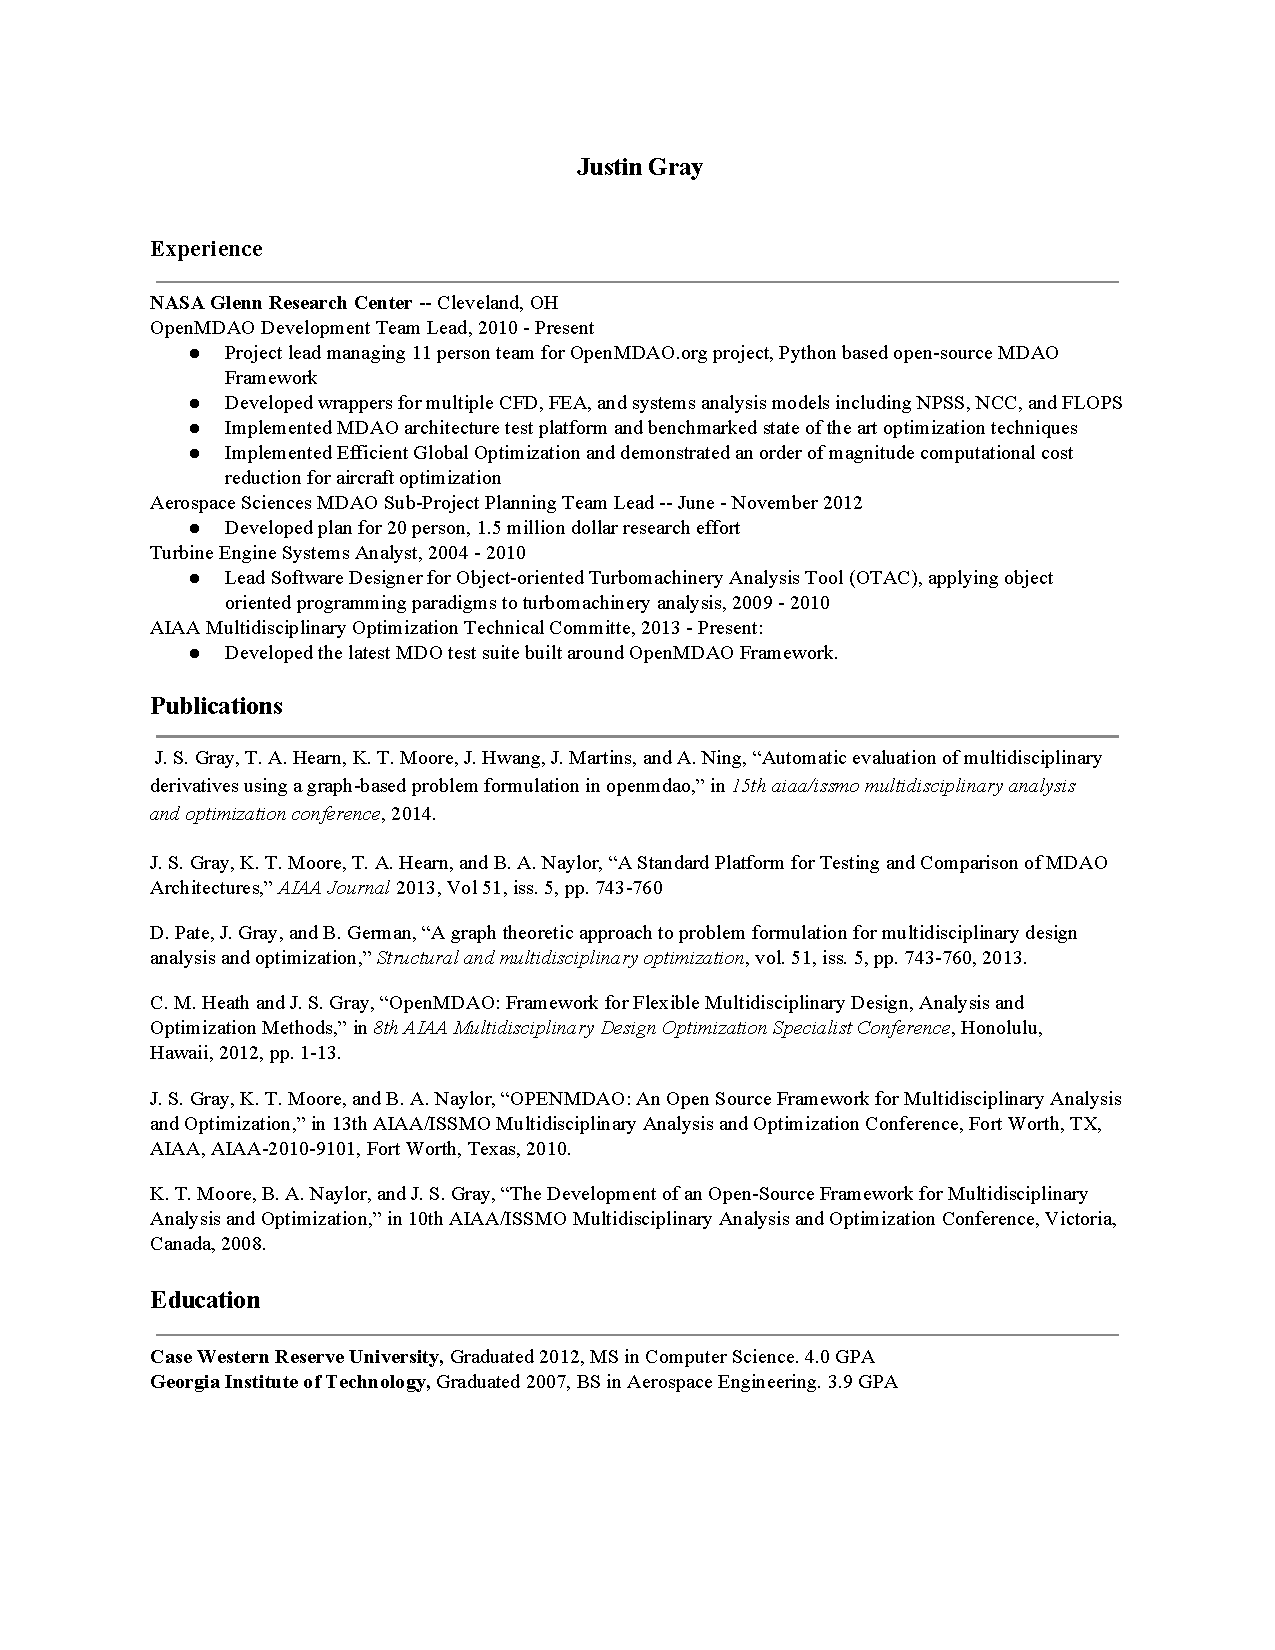
\includepdf[pages={1}]{resumes/justin_resume.pdf}
  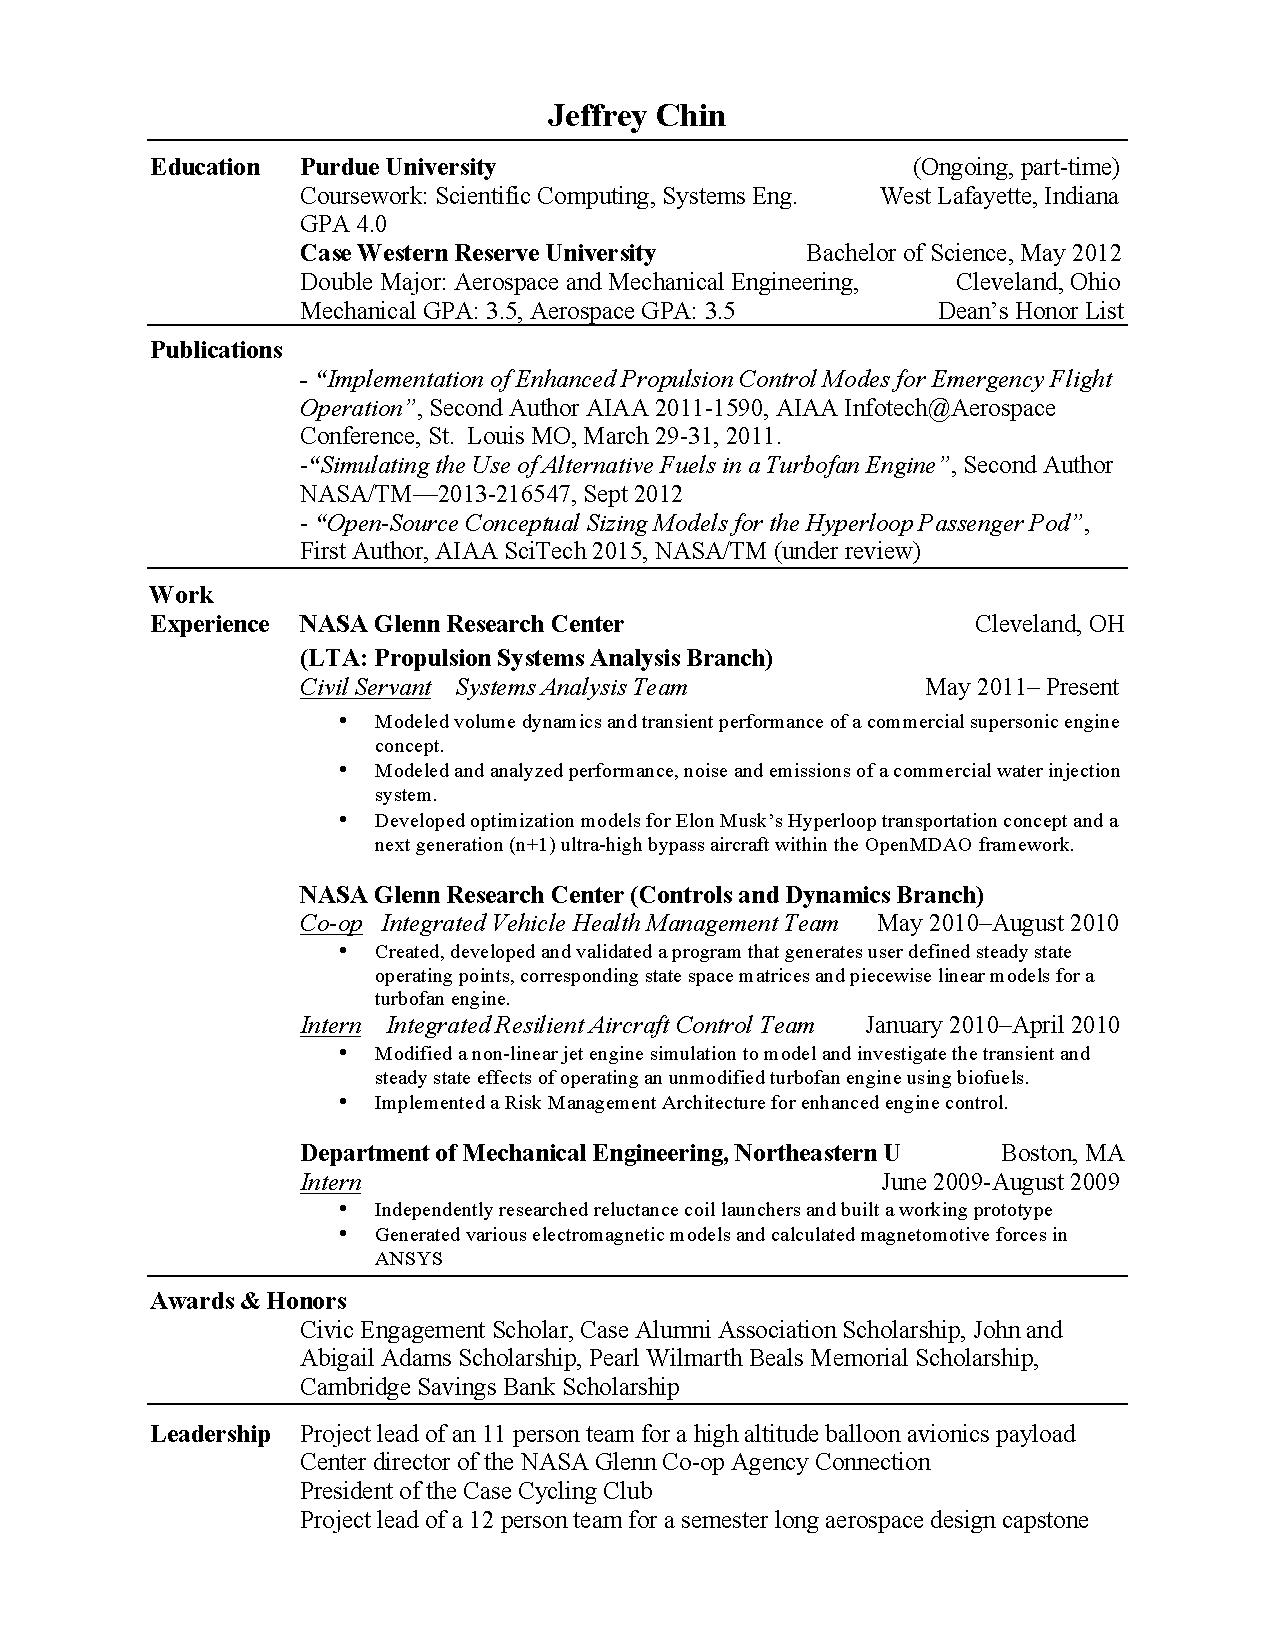
\includepdf[pages={1}]{resumes/Chin_SeedlingResume9_3_14.pdf}


\end{document}
